\documentclass[]{article}

\usepackage{sbc2001}

\usepackage[utf8]{inputenc}
\usepackage{amssymb,amsmath}
\usepackage[portuges,brazil]{babel}
\usepackage{boxedminipage}
\usepackage{listings}
\usepackage{ifpdf}
\usepackage{longtable}
\usepackage{url}

\ifpdf
\usepackage[pdftex]{graphicx}
\else
\usepackage{graphicx}
\fi

\newcommand{\HRule}{\rule{\linewidth}{1mm}}

\begin{document}

\date{Julho 22, 2010}   

\sloppy

\title{\emph{Design Patterns - Factory Method}}
\author{Fabricio Griebler, Manuela Valente, Marlon Lopes}

\address{
         %%Pós-Graduação \\
	 Especialização em Tecnologias Aplicadas a Sistemas de Informação com Métodos Ágeis - 4ª Edição \\
         Uniritter \\
         Porto Alegre, RS \\
         \email{fabricio@fasagri.com.br, valente.manu@gmail.com,
marlonglopes@gmail.com}
}

\maketitle

\pagestyle{plain}
\pagenumbering{roman}


\begin{resumo}

Este artigo apresenta uma descrição sucinta do padrão de projetos orientado a objetos chamado Factory Method (Método de Fabrica), 

\end{resumo}


\begin{abstract}


\end{abstract}

\pagenumbering{arabic}
\setcounter{page}{1}

\section{Introdução}
\label{sec:introducao}
\subsection{O que é um padrão de design (\emph{Design Pattern})}
\label{sub:introducao}

Cada padrão descreve um problema que ocorre ao longo do tempo
mais de uma vez em nosso meio, e então descreve o núcleo da solução
para esse problema, de tal forma que você pode usar esta solução um milhão de vezes
mais, sem nunca fazê-lo da mesma forma duas vezes. 
Mesmo que se estivesse falando em padrões de construção de edifícios, também é verdade para padrões de construção de software orientado a objeto. Nossas soluções são expressas em termos de objetos e interfaces em vez de paredes e portas, mas no cerne dos dois tipos de padrões existe uma solução para um problema em um contexto.\cite{gamma95}

Em geral, um padrão tem quatro elementos essenciais:\cite{gamma95}

\begin{enumerate}
	\item 

O \textbf{nome do padrão} é um identificador que podemos usar para descrever um problema de \emph{design}, suas
soluções, e suas consequências em uma ou duas palavras. A nomeação de um padrão imediatamente
aumenta o nosso vocabulário de design. Ela nos permite projetar em um nível mais elevado de
abstração. Ter um vocabulário de padrões permite-nos falar sobre eles com
nossos colegas, em nossa documentação, e até mesmo para nós mesmos. Torna-se
mais fácil pensar sobre os projetos e comunicar-se com as pessoas envolvidas. Encontrar bons nomes tem sido uma das partes mais difíceis de desenvolver nosso catálogo.

	\item 


O \textbf{problema} descreve quando aplicar o padrão. Ele explica o problema
e seu contexto. Poderia descrever os problemas específicos de design tais como
como representar algoritmos como objetos. Poderia descrever classe ou
estruturas de objeto que são sintomáticas de um projeto inflexível. Às vezes, a
problema irá incluir uma lista de condições que devem ser cumpridas antes que faça
sentido de aplicar o padrão.


	\item 


A \textbf{solução} descreve os elementos que compõem o projeto, suas
relações, responsabilidades e colaborações. A solução não
descreve um determinado design concreto ou de execução, porque um padrão
é como um modelo que pode ser aplicado em muitas situações diferentes. Em vez disso,
o padrão fornece uma descrição abstrata de um problema de projeto e como
um regime geral de elementos (classes e objetos no nosso caso) resolve
ele.

	\item 


As \textbf{consequências} são os resultados da aplicação do modelo.
Quando descrevemos as decisões de design, eles são críticos para avaliar alternativas de projeto e para a compreensão
dos custos e benefícios da aplicação do modelo. As consequências para o
software são preocupação com freqüência e tempo de execução. Podem sinalizar linguagem
e questões de implementação. Uma vez que a reutilização é frequentemente um fator de
\emph{design} orientado a objeto, as conseqüências de um padrão inclui o seu impacto
sobre a flexibilidade de um sistema, extensibilidade ou portabilidade. Listando estas
conseqüências explicitamente ajuda você a compreender e avaliá-los.


\end{enumerate}

\subsection{\emph{Design Patterns} existentes}
\label{sub:designexistentes}


Os padrões hoje existentes estão divididos em três grupos:\cite{gamma95}

\begin{itemize}
	\item
		Padrões de criação (\emph{Creational patterns}) \\

		\begin{itemize}
			\item 
				\emph{Abstract factory}, Fornece uma interface para criar famílias de objetos relacionados ou dependentes sem especificar suas classes concretas.\\

			\item 
				\emph{Builder}, Separa a construção de um objeto complexo da sua representação para que
o mesmo processo de construção possa criar diferentes representações.\\
			\item 
				\emph{Factory method}, Define uma interface para criar um objeto, mas deixa as subclasses decidirem qual classe instanciar. \emph{Factory Method} permite subclasses façam a instanciação.\\

			\item 
				\emph{Prototype}, Especifica o tipo de objectos a criar usando uma instância de protótipo, e cria
novos objetos copiando este protótipo.\\

			\item 
				\emph{Singleton}, Certifica-se de que uma classe tem apenas um exemplo, e fornece um ponto global de acesso à ele.\\

		\end{itemize}

	\item
		Padrões estruturais (\emph{Structural patterns})\\
		
		\begin{itemize}
			\item \emph{Adapter}, Converte a interface de uma classe para outra interface que os clientes esperam. Este adaptador permite que classes trabalhem em conjunto, de outro modo não seria possivel por causa da incompatibilidade
interfaces.  \\
			\item \emph{Bridge}, Desacopla uma abstração de sua implementação para que as duas possam variar
de forma independente.\\

			\item \emph{Composite}, Tem o objetivo de compor objetos em estruturas de árvore para representar hierarquias parte-todo. \emph{Composite} permite que clientes tratem objetos individuais e composições de objetos
uniformemente.\\

			\item
				\emph{Decorator}, Anexa responsabilidades adicionais a um objeto dinamicamente. \emph{Decorators} fornecem uma alternativa flexível a subclasses para extensão da funcionalidade.\\

			\item \emph{Facade}, Fornece uma interface unificada para um conjunto de interfaces em um subsistema. \emph{Facade} define uma interface de alto nível que torna o subsistema mais fácil de usar.\\

			\item \emph{Flyweight}, Usa compartilhamento para suportar um grande número de objetos de forma eficiente.\\

			\item \emph{Proxy}, Proporciona um espaço para outro objeto para controlar o acesso a ele.\\


		\end{itemize}

	\item
		Padrões comportamentais (\emph{Behavioral patterns})\\

		\begin{itemize}
			\item \emph{Chain of Responsibility}, Evita o acoplamento do remetente de um pedido de seu receptor, dando a mais de um objeto a oportunidade para manipular a solicitação. Faz com que a cadeia os objetos e passe a receber pedido até que um objeto gere.\\

			\item \emph{Command}, Encapsula uma solicitação como um objeto, assim permitindo parametrizar clientes com
diferentes pedidos, cria fila ou solicitações de log e suporte às operações reversível.\\

			\item \emph{Interpreter}, Dada uma linguagem, define uma representação para sua gramática juntamente com um intérprete que usa a representação para interpretar sentenças na linguagem.\\

			\item \emph{Iterator}, Fornece uma maneira de acessar os elementos de um objeto agregado seqüencialmente sem expor sua representação subjacente.\\

			\item \emph{Mediator}, Define um objeto que encapsula como um conjunto de objetos \emph{interact.Mediator} promove acoplamento, mantendo os objetos de cada EPI referindo explicitamente outros, e ele permite que você varie sua interação de forma independente.\\


			\item \emph{Memento}, Sem violar o encapsulamento, captura e externaliza o estado de um \emph{object sinternal} para que o objeto pode ser restaurado para este estado mais tarde. \\

			\item \emph{Observer}, Define uma dependência um-para-muitos entre objetos de modo que quando um objeto muda de estado, todos seus dependentes sejam notificados e atualizados automaticamente.\\

			\item \emph{State}, Permite que um objeto altere seu comportamento quando seu estado interno muda.\\
			
			\item \emph{Strategy}, Define uma família de algoritmos, encapsula cada um, e torna-os intercambiáveis.
Esta estratégia permite que o algoritmo pode variar independentemente do cliente que usá-lo.\\


			\item \emph{Template Method}, Define o esqueleto de um algoritmo numa operação, adiando alguns passos para as subclasses. Permite que subclasses redefinam certos passos de um algoritmo sem alterar a estrutura do algoritmo.\\

			\item \emph{Visitor}, Representa uma operação a ser realizada sobre os elementos de uma estrutura de objetos. Permite que você defina uma nova operação sem alterar as classes dos elementos em que opera.\\



		\end{itemize}

\end{itemize}

Estes são os padrões mais comumente utilizados, neste trabalho será detalhado o Padrão de criação \emph{Factory Method}, tambem conhecido como \emph{Virtual Constructor} (Construtor virtual).


\section{\emph{Factory Method}}
\label{sec:factory1}
O padrão \emph{Factory Method} está relacionado a todos os outros padrões que conduzam
algum tipo de construção encapsulada de objetos. Além de \emph{factory} os padrões Iterator,
Singleton , Builder, Prototype e Bridge- para citar alguns – estão relacionados ao padrão
\emph{Factory Method}.

Define uma interface para a criação de um objeto, mas deixa que as subclasses
decidam qual a classe instanciar. Permite a uma classe delegar a instanciação para as
subclasses.\cite{gamma95}


\subsection{Motivação}
\label{sub:fac_motiv}

\emph{Frameworks} usam classes abstratas para definir e manter relacionamentos entre
objetos. Um \emph{framework} é muitas vezes responsável por criar esses objetos também.

Considere-se um \emph{framework} de aplicações que podem apresentar vários documentos ao
usuário. Duas abstrações chave neste \emph{framework} são as classes Application e
Documento. Ambas as classes são abstratas, e os clientes têm usalas como subclasses para perceber
suas implementações de aplicações específicas. Para criar um aplicativo de desenho, por
exemplo, podemos definir as classes e \emph{DrawingApplication} e \emph{DrawingDocument}. A
classe Application é responsável pela gestão de documentos e como criá-los assim que o usuário selecione Open ou Novo a partir de um menu, por exemplo.\cite{gamma95}

Como subclasse do documento em particular para instanciar é específico do aplicativo,
a classe Application não consegue prever que documento deve criar, a classe Application só sabe quando um novo documento deve ser criado, não o tipo do documento para criar. Isso cria um dilema: O \emph{framework} deve instanciar classes, mas só sabe sobre classes abstratas, que não pode instanciar.\cite{gamma95}

O padrão \emph{Factory Method} oferece uma solução. Ele encapsula o conhecimento de
que subclasse Documento deve criar e move este conhecimento para fora do \emph{framework}.\cite{gamma95}

\begin{center}
	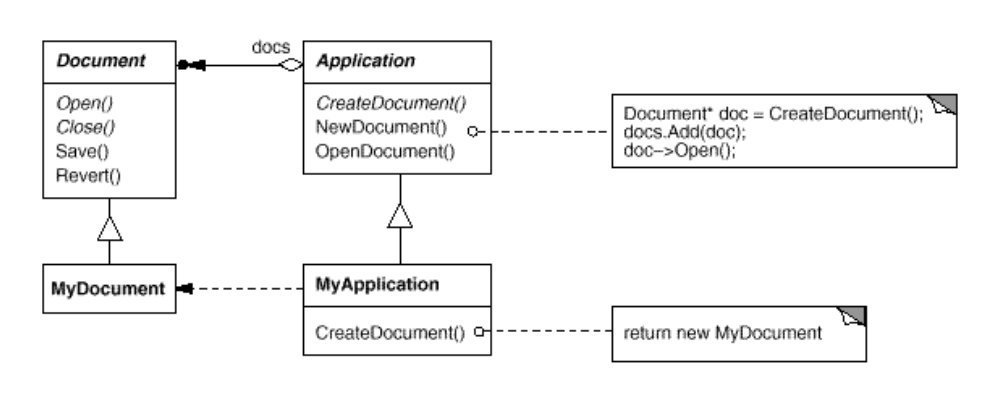
\includegraphics[scale=0.40]{Figuras/image1.jpg}
	\captionof{figure}{\label{diagrama1} Representação da estrutura para criação de documentos}
	\label{fig:diagrama1}
\end{center}

As subclasses da aplicação redefinem uma operação abstrata \emph{CreateDocument} no 
aplicativo para retornar a subclasse apropriada documento. Uma vez que uma subclasse da aplicação é instanciada, ele pode então instanciar documentos sem saber sua classe. Chamamos \emph{CreateDocument} um \emph{factory method} porque é
responsável por "produzir" um objeto.\cite{gamma95}

\subsection{Aplicação}
\label{sub:fac_aplica}

Se usa \emph{Factory pattern} quando:\cite{gamma95}

\begin{itemize}
	\item Quando uma classe (o criador) não pode antecipar a classe dos objetos que deve criar.
.	\item Quando Uma classe quer que suas subclasses possam especificar os objetos que ele cria.
	\item Quando classes delegam responsabilidade para uma entre várias subclasses de apoio e
queremos localizar num ponto único a conhecimento de qual subclasse está sendo usada.

\end{itemize}


\subsection{Problema}
\label{sub:fac_problema}

Uma classe precisa instanciar a derivação de uma outra, mas não sabe qual. O \emph{Factory Method} permite que uma classe derivada tome essa decisão.

\subsection{Solução}
\label{sub:fac_solucao}

Uma classe derivada decide qual classe instanciar e o modo como instanciá-la.
Algumas razões existem para que não queria utilizar new diretamente. A primeira, e
mais óbvia, é não saber que classe de objeto instanciar.
Isso é comum numa aplicação bem desenhada onde variáveis são estruturadas com
base em interfaces. Assim, vários tipos de objetos diferentes podem ser associados a
essa variável. Outra razão é a necessidade de inicializar o objeto instanciado antes de ser
atribuído à variável. Importante notar
que esta inicialização não depende do ambiente onde o objeto será utilizado, mas apenas
da estrutura do próprio objeto.\cite{fact1}\cite{gamma95}



\subsection{Como utilizar}
\label{sub:fac_utilizacao}

\begin{itemize}
	\item É possível criar um objeto sem ter conhecimento algum de sua classe concreta?
	\item Esse conhecimento deve estar em alguma parte do sistema, mas não precisa estar
no cliente
	\item \emph{FactoryMethod} define uma interface comum para criar objetos
	\item O objeto específico é determinado nas diferentes implementações dessa interface
	\item O cliente do \emph{FactoryMethod} precisa saber sobre implementações concretas do
objeto criador do produto desejado

\end{itemize}


\subsection{Diagrama de classes}
\label{sub:fac_diagrama}

\begin{center}
	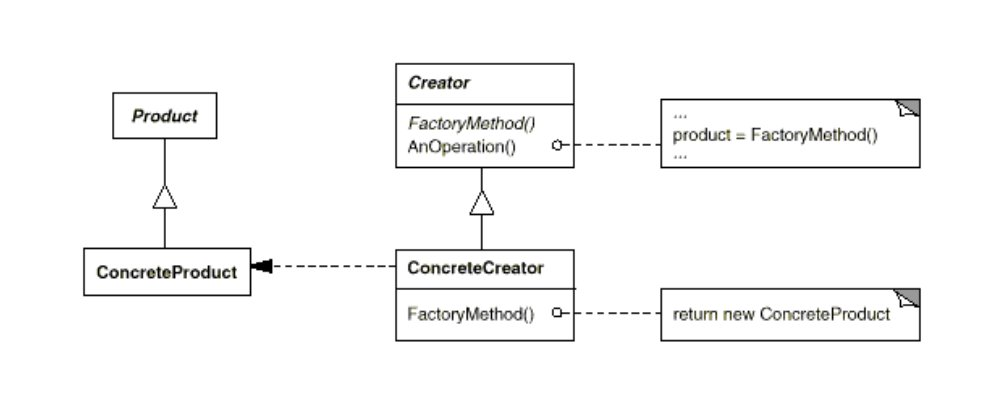
\includegraphics[scale=0.40]{Figuras/image2.jpg}
	\captionof{figure}{\label{diagrama2} Representação da estrutura de classes utilizando \emph{factory method}}
	\label{fig:diagrama2}
\end{center}

\begin{itemize}
	\item \emph{Product}: define a interface dos objetos criados pelo \emph{Factory Method}
	\item \emph{ConcreteProduct}: implementa a interface \emph{Product}
	\item \emph{Creator}: declara o \emph{Factory Method} que retorna um objeto do tipo \emph{Product}
		\begin{itemize}
			\item  Às vezes, o \emph{Creator} não é apenas uma interface, mas pode envolver uma
classe concreta que tenha uma implementação default para o \emph{Factory Method} para retornar um objeto com algum tipo \emph{ConcreteProduct} default
			\item Pode chamar o \emph{Factory Method} para criar um produto do tipo \emph{Product}
		\end{itemize}
	\item \emph{ConcreteCreator}: faz override do \emph{Factory Method} para retornar uma instância de \emph{ConcreteProduct}
\end{itemize}

O criador confia em suas subclasses para definir o \emph{Factory Method} que retorne uma instância da \emph{ConcreteProduct} adequado.


\subsection{Consequencias e benefícios}
\label{sub:fac_conse+benef}

\emph{Factory Method} elimina a necessidade de vincular as classes específicas do aplicativo em seu código. O código lida apenas com a interface \emph{Product}, pois pode trabalhar com qualquer classe \emph{ConcreteProduct} definida pelo usuário.

Uma desvantagem potencial do \emph{factory method} é que os clientes podem precisar ter uma subclasse \emph{Creator} apenas para criar um objeto \emph{ConcreteProduct} específico.

Se o cliente tem que criar de qualquer maneira uma subclasse da classe \emph{Creator}, usar subclasses pode ser uma boa solução, mas de outra maneira o cliente tem que lidar com outro ponto da evolução.

Aqui estão duas consequências adicionais do padrão \emph{Factory Method}:

\begin{enumerate}
	\item Fornecer ganchos para subclasses. Criação de objetos dentro de uma classe com \emph{factory methods} é sempre mais flexível do que criar um objeto diretamente. \emph{Factory Method} da para subclasses um gancho para fornecer uma versão estendida
de um objeto.

No exemplo do documento, a classe \emph{Document} poderia definir um \emph{factory method} chamado \emph{CreateFileDialog} que cria uma caixa de dialogo padrão na abertura de documentos existentes.

Uma subclasse \emph{Document} pode definir uma caixa de dialogo específico do aplicativo, substituindo este \emph{factory method}. Neste caso, o \emph{factory method} não é abstrato, mas fornece implementação default.

	\item
\end{enumerate}

\begin{itemize}
	\item Criação de objetos é desacoplada do conhecimento do tipo concreto do objeto
	\item Conecta hierarquias de classe paralelas
	\item Facilita a extensibilidade
\end{itemize}

\emph{Factory Methods} eliminam a necessidade de colocar classes específicas da aplicação no código.\cite{fact2}

\begin{itemize}
	\item O código só lida com a interface \emph{Product}
	\item O código pode, portanto funcionar com qualquer classe \emph{ConcreteProduct} Provê ganchos (\emph{Hook Methods}) para subclasses.
	\item Criar objetos dentro de uma classe com um \emph{Factory Method} é sempre mais flexível do que criar objetos diretamente.
	\item O \emph{Factory Method} provê um gancho para que subclasses forneçam uma versão estendida de um objeto
\end{itemize}


\subsection{Exemplos de uso}
\label{sub:fac_uso}



\bibliographystyle{abnt}

\renewcommand{\bibname}{Referência Bibliografia}
\bibliography{references}

\end{document}
